%
% File lfd1617.tex
%
%% Based on the style files for EACL-2017
%% Based on the style files for ACL-2016
%% Based on the style files for ACL-2015, with some improvements
%%  taken from the NAACL-2016 style
%% Based on the style files for ACL-2014, which were, in turn,
%% Based on the style files for ACL-2013, which were, in turn,
%% Based on the style files for ACL-2012, which were, in turn,
%% based on the style files for ACL-2011, which were, in turn,
%% based on the style files for ACL-2010, which were, in turn,
%% based on the style files for ACL-IJCNLP-2009, which were, in turn,
%% based on the style files for EACL-2009 and IJCNLP-2008...

%% Based on the style files for EACL 2006 by
%%e.agirre@ehu.es or Sergi.Balari@uab.es
%% and that of ACL 08 by Joakim Nivre and Noah Smith

\documentclass[11pt]{article}
\usepackage{eacl2017}
\usepackage{times}
\usepackage{url}
\usepackage{latexsym}
\usepackage{tikz}
\usepackage{pgfplots}
\pgfplotsset{compat=1.14}

%%%% LEAVE THIS IN
\eaclfinalcopy


\newcommand\BibTeX{B{\sc ib}\TeX}



\title{Learning from Data - Assignment 3 - Support Vector Machines and K-Means}

\author{Remko Boschker \\
  master student of information science at the Rijks Universiteit Groningen \\
  {\tt s1282603, r.boschker@student.rug.nl} }

\date{}

\begin{document}
\maketitle
\begin{abstract}

\end{abstract}

\section{Introduction}



\section{Data}

The study uses a corpus of six thousand product reviews. Each review consists of a label indicating whether the review is positive or negative and a label indicating to which of the followings six topics it belongs: books, camera, dvd, health, music or software. The review also contains a file reference and the actual text of the review. The topic and sentiment labels are distributed almost equally across the corpus. About half of the reviews about a particular topic are labeled positive. Table~\ref{tab:corpus} shows the counts for the labels in the corpus.

\begin{table}[ht]\footnotesize
\caption{counts of topic and sentiment labels}
\label{tab:corpus}
\begin{tabular}{ l r r r r r r }
topic & cnt & \% & pos & \% & neg & \% \\
\hline
books & 993 & 16.5 & 471 & 47 & 522 & 53 \\
music & 1027 & 17.1 & 531 & 52 & 496 & 48 \\
dvd & 1012 & 16.9 & 490 & 48 & 522 & 52 \\
health & 986 & 16.4 & 470 & 48 & 516 & 52 \\
software & 994 & 16.6 & 502 & 51 & 492 & 49 \\
camera & 988 & 16.5 & 504 & 51 & 484 & 49 \\
\hline
total & 6000 & 100.0 & 2968 & 48 & 3132 & 52 \\
\end{tabular}

\end{table}

I also use a subset of the Reuters Corpus Volume 1 (RCV1, http://www.daviddlewis.com/ resources/testcollections/rcv1/). It was created by Zhi Liu (National Engineer- ing Research Center for E-Learning, Hubei Wuhan, China). The top 50 authors (with respect to total size of articles) were selected, and for each of them 50 articles were picked that have at least one subtopic of the class CCAT(corporate/industrial). This is a way to minimise the topic factor in distinguishing among the texts. The training corpus consists of 2,500 texts (50 per author); the test corpus also includes 2,500 texts (50 per author), non-overlapping with the training texts.

\section{K-Means}

K-Means is an unsupervised machine learning algorithm to cluster similar samples together in a vector space. I run the algorithm on the review data with the \emph{k}-value equal to 6 to evaluate performance in classifying the reviews by topic. I experiment with changing the number of times the algorithm is run with different seed centroids. I use no preprocessor and the tf-idf vectoriser. Next I run the algorithm on a subset of the review data containing only two topics. I try to steer the outcome of the clustering towards either grouping the topics or the sentiment labels together by using feature selection based on the variance threshold or on selecting the best features with regards to \emph{f}, \emph{$chi^2$} and mutual information measures. Thirdly I run the clustering algorithm on the author data to try and cluster the texts from the same author together. I try different combinations of word and character n-gram vector representations as well as part of speech tags. Performance of the clustering will be evaluated on Rand Index and V-Measure scores using four-fold cross-validation. For the author clustering task I evaluate the configuration with the highest score with unseen test data.

\begin{figure}
  \caption{plot of Rand Index and V-Measure for different numbers of times the algorithm was run with different centroid seeds}
  \label{fig:k-seeds}
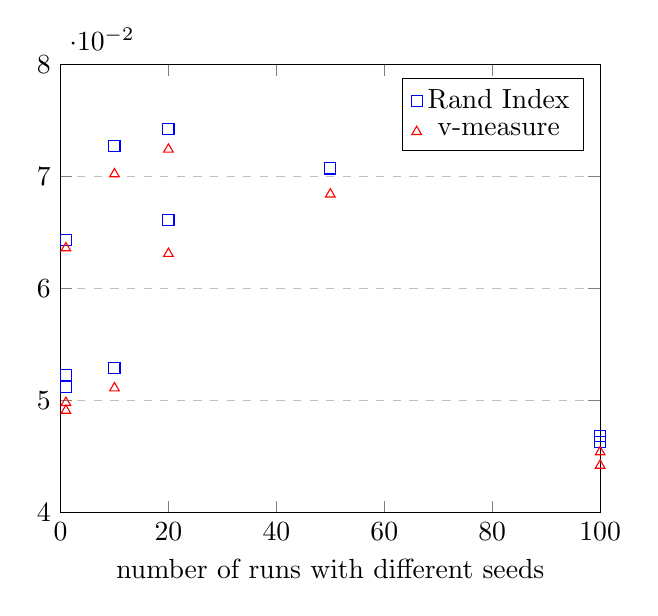
\begin{tikzpicture}

	\begin{axis}[
    title={},
    xlabel={number of runs with different seeds},
    ylabel={},
    xmin=0, xmax=100,
    ymin=0.04, ymax=0.08,
    legend pos=north east,
    ymajorgrids=true,
    grid style=dashed,
	]
  \addplot [
    only marks,
    color=blue,
    mark=square,
    ] coordinates {
    (1  , 0.0643)
    (1  , 0.0512)
    (1  , 0.0523)
    (10 , 0.0529)
    (10 , 0.0727)
    (20 , 0.0661)
    (20 , 0.0742)
    (50 , 0.0384)
    (50 , 0.0707)
    (100, 0.0463)
    (100, 0.0468)
  };
  \addlegendentry{Rand Index}

	\addplot [
    only marks,
    color=red,
    mark=triangle,
    ] coordinates {
    (1  , 0.0636)
    (1  , 0.0498)
    (1  , 0.0491)
    (10 , 0.0511)
    (10 , 0.0702)
    (20 , 0.0631)
    (20 , 0.0724)
    (50 , 0.0373)
    (50 , 0.0684)
    (100, 0.0442)
    (100, 0.0454)
	};
	\addlegendentry{v-measure}
	\end{axis}
\end{tikzpicture}
\end{figure}

Figure~\ref{fig:k-seeds} plots the Rand Indices and V-Measures for different numbers of runs of the k-means algorithm on the review data with \emph{k} equals 6 and evaluation against the topic labels. Each run the algorithm is initialised with different seed centroids that the samples cluster around. The run with the lowest resulting inertia, inter-cluster sum of squares, is selected as the best run. I expected a higher number of runs to result in a clustering with higher scores. For different runs of the experiment with identical settings the resulting scores vary to a similar extend as between experiments runs with a different number of seedings. Therefore I can only conclude that the clustering is unstable. In general both the Rand Index and V-Measure show that most reviews are in the wrong cluster and that clusters contain many reviews that have a label different from the one assigned to the cluster. Comparing the golden labels of reviews assigned to a particular cluster confirms this as well.

\begin{table}[ht]\footnotesize
\centering
\caption{scores for feature selection in clustering topic or sentiment}
\label{tab:clust-select}
\begin{tabular}{ l r r }
selector & RI topic & RI sentiment \\
\hline
none           & 0.0965 & 0.0006 \\
variance 0     & 0.0288 & 0.0003 \\
variance 1e-6  & 0.0231 & 0.0002 \\
10  best F     & 0.4904 & 0.0205 \\
10  best MI    & 0.0561 & 0.0002 \\
10  best Chi2  & 0.0104 & 0.0000 \\
100 best F     & 0.0106 & 0.0017 \\
100 best MI    & 0.0141 & 0.0006 \\
100 best Chi2  & 0.0369 & 0.0005 \\
\end{tabular}
\end{table}

I take a subset of the review data that contains only reviews of cameras and of music. With the number of clusters set to two I try to steer the clustering towards either clustering the reviews with a positive or negative sentiment together or clustering the reviews about cameras or about music together. My assumption is that sentiment is conveyed by less specific words than topic. Selecting features based on various tests related to variance could influence the clustering. I try setting a variance threshold of \emph{1e-5} and \emph{1e-6} and I try selecting the k-best features for \emph{k} equal to \emph{5, 10, 20, 50, 100, 250} based on \emph{ANOVA F-value}, \emph{$chi^2$ statistics} and on \emph{Mutual Information}. The scores for evaluating on the topic labels continue to be much higher than on the sentiment labels. Some of the resulting scores can be found in table~\ref{tab:clust-select}. Selecting features tends to increase the difference in scoring. This somewhat supports the assumption. Because the clustering is already greatly in favour of the topic labels it does not help me in steering the clustering towards the sentiment labels.

\begin{table}[ht]\footnotesize
\centering
\caption{scores for author clustering for different features}
\label{tab:authors}
\begin{tabular}{ l r r }
features & RI & V-measure \\
\hline
word \{n=1,2\}            & 0.6633 & 0.5755 \\
word \{n=1,2\}            & 0.6725 & 0.5687 \\
word \{n=1,2\} + char \{n=5\} & 0.6511 & 0.5685 \\
word \{n=1,2\} + POS      & 0.5703 & 0.5325 \\
char \{n=5\}              & 0.6554 & 0.5691 \\
word \{n=1,2,3\} lemma    & 0.6614 & 0.5712 \\
word \{n=1,2,3\} stemmed  & 0.6435 & 0.5663 \\
word \{n=3\}              & 0.6520 & 0.5685 \\
\end{tabular}
\end{table}

The last set of experiments with k-means clustering uses the author corpus described in the data section of this report. There are fifty authors and therefore the number of clusters is set at fifty. I vary the features used by the algorithm. I use tf-idf vectors with word n-grams, character n-grams and part-of-speech labels. I list the Rand Index and V-Measure scores for cross-validation on the development data in table~\ref{tab:authors}. The differences between the various n-gram features are small and including the part-of-speech tags has a negative impact. Also here the clustering is not stable and it is hard to draw any conclusions from this data. The word uni+bigram is fastest and it seems to score slightly higher. I evaluate it on the test data to find a Rand Index of \textbf{0.7011} and a V-Measure of \textbf{0.5854}.

\section{Support Vector Machines}

I use a SVM to perform binary classification of the review data into reviews with a positive or negative sentiment. I evaluate the influence of the soft-margin constant \emph{C} and use both a linear and a radial basis kernel function. For the radial basis kernel function I evaluate different values for \emph{$\gamma$}, the inverse of how far the influence of a sample selected as a support vector reaches. I next try to find the best performance by evaluating different combinations of features including clustering based features. Performance is evaluated on the f1-score of the classification using four-fold cross-validation.

\begin{figure}
  \caption{f1-scores for differenct c-values}
  \label{fig:c-val}
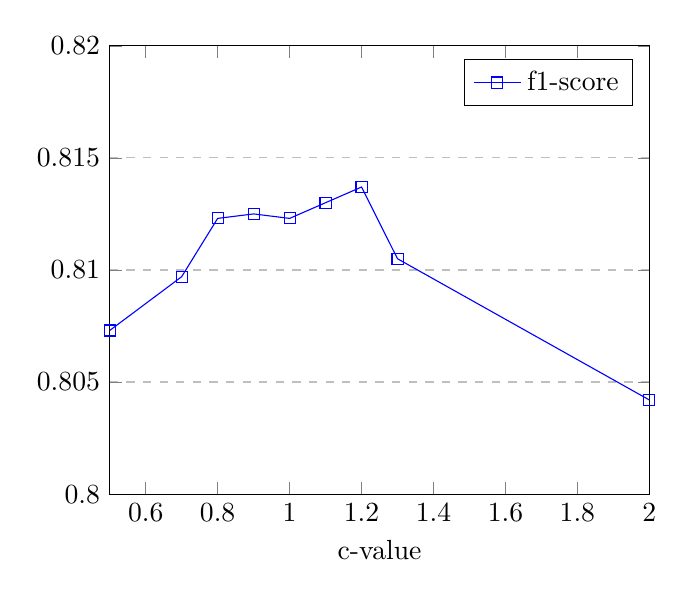
\begin{tikzpicture}

	\begin{axis}[
    title={},
    xlabel={c-value},
    ylabel={},
    xmin=0.5, xmax=2.0,
    ymin=0.800, ymax=0.820,
    legend pos=north east,
    ymajorgrids=true,
    grid style=dashed,
    yticklabel style={/pgf/number format/precision=3},
	]
  \addplot [
    color=blue,
    mark=square,
    ] coordinates {
      (0.5, 0.8073)
      (0.7, 0.8097)
      (0.8, 0.8123)
      (0.9, 0.8125)
      (1.0, 0.8123)
      (1.1, 0.8130)
      (1.2, 0.8137)
      (1.3, 0.8105)
      (2.0, 0.8042)
    };
\addlegendentry{f1-score}
\end{axis}
\end{tikzpicture}
\end{figure}

The c-value, the soft margin constant, determines the error penalty for samples that are close to the separating hyperplane. If the c-value is higher the SVM optimisation will choose a smaller margin to classify samples correctly. But if the margin is smaller the chance that new data is misclassified is greater. Figure~\ref{fig:c-val} plots the f1-score for c-values around the default value of 1.0. A c-value of \textbf{1.2} scores the highest.

\begin{figure}
  \caption{f1-scores for $\gamma$ values for a rbf kernel and a c-value of 1.0}
  \label{fig:c-val}
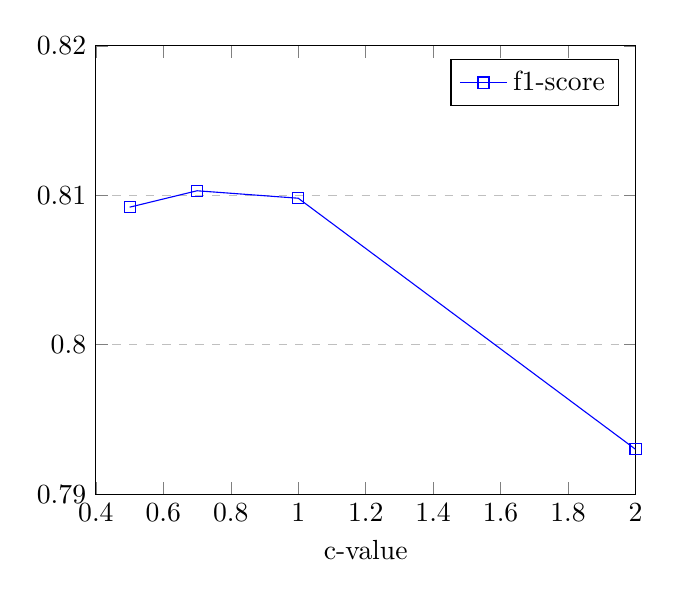
\begin{tikzpicture}

	\begin{axis}[
    title={},
    xlabel={c-value},
    ylabel={},
    xmin=0.4, xmax=2.0,
    ymin=0.790, ymax=0.820,
    legend pos=north east,
    ymajorgrids=true,
    grid style=dashed,
    yticklabel style={/pgf/number format/precision=3},
	]
  \addplot [
    color=blue,
    mark=square,
    ] coordinates {
      (0.5, 0.8092)
      (0.7, 0.8103)
      (1.0, 0.8098)
      (2.0, 0.7930)
    };
\addlegendentry{f1-score}
\end{axis}
\end{tikzpicture}
\end{figure}

Linear kernel are supposed to work best for text classification tasks. However when I run the SVM algorithm with a radial basis function kernel it performs as well as with the linear kernel. I first investigate the influence of the kernel coefficient $\gamma$. This coefficient determines the sensitivity of the optimisation to differences in input vectors. The precise impact is dependent on dimensionality and normalisation. Figure~\ref{fig:gamma} shows the impact of tuning the $\gamma$-value with the c-value set to 1.0. Tuning the c-value together with the $\gamma$-value leads to a maximum f1-score of \textbf{0.8153} at a c-value of \textbf{1.4} and a $\gamma$-value of \textbf{0.9}.





lemmatise 0.8158    0.8157    0.8157
word bigram 0.8188    0.8188    0.8188
bigram only 0.7650    0.7645    0.7643
word trigram 0.8081    0.8078    0.8077
trigram only 0.6704    0.6703    0.6703
count vect 0.5234    0.5207    0.4915
char trigram only 0.8178    0.8178    0.8178
char 3,4gram 0.8323    0.8323    0.8323
char 4 gram
char 3,4,5gram 0.8410    0.8410    0.8410
char 5 grm 0.8482    0.8482    0.8482
char 6 grm 0.8514    0.8513    0.8513
linear 0.9 0.8525    0.8525    0.8525
charwb 6 0.8270    0.8270    0.8270
word tags 0.8525    0.8525    0.8525
seq tag 0.8475    0.8475    0.8475
with cluster 0.8532    0.8532    0.8531


\section{Discussion/Conclusion}




\bibliography{eacl2017}
\bibliography{yourbibfile}

\end{document}
